\documentclass[preprint]{sigplanconf}[10pt]

% The following \documentclass options may be useful:
%
% 10pt          To set in 10-point type instead of 9-point.
% 11pt          To set in 11-point type instead of 9-point.
% authoryear    To obtain author/year citation style instead of numeric.

\usepackage{amsmath}
\usepackage{graphicx}
\usepackage{mathpartir} % To use \inferrule
\usepackage{amssymb}    % To use \mathbb

\newtheorem{definition}[section]{Definition}

% Definition of new commands that I use in this text:
\newcommand{\fun}[1]{\mbox{\textbf{#1}}}
\newcommand{\lb}[1]{#1_{\downarrow}}
\newcommand{\ub}[1]{#1_{\uparrow}}
\newcommand{\varset}[1]{\mbox{$\cal{#1}$}}
\newcommand{\code}[1]{\textbf{#1}}

\begin{document}

\conferenceinfo{CGO '13}{February 23 - February 27. Shenzhen, China} 
\copyrightyear{2013}
\copyrightdata{[to be supplied]} 

\titlebanner{Dinamica EGO}        % These are ignored unless
\preprintfooter{Dinamica EGO}   % 'preprint' option specified.

\title{An Algorithm to Prune Integer Overflow Tests}
%\subtitle{A case study of the Dinamica EGO toolkit}

\authorinfo{Removed due to blind review}
           {No affiliation given}
           {No e-mail given}

\maketitle

\begin{abstract}
The integer primitive type has upper and lower bounds in many programming
languages, including C, C++ and Java.
This limitation might lead programs that manipulate large integer numbers to
produce unexpected results due to overflows.
There exists a plethora of works that instrument programs to track the occurrence
of these overflows.
In this paper we present an algorithm that relies on static range analysis to
eliminate this instrumentation whenever possible.
We present a novel live range splitting strategy that refine the precision of
our range analysis.
We have used this algorithm to improve the quality of a dynamic instrumentation
library that we have implemented in LLVM.
This framework has been used to detect overflows in hundreds of C/C++ programs.
As a testimony of its effectiveness, our range analysis has been able to speedup
the SPEC CPU 2006 instrumented programs by XX\%.
\end{abstract}

\category{D.3.4}{Processors}{Compilers}

\terms
Languages, Performance

\keywords
Integer arithmetics, Overflow, Compiler, Range analysis

\section{Introduction}
\label{sec:int}

% What are integer overflows.
The most popular programming languages, including C, C++ and Java, limit the
size of primitive numeric types.
For instance, the \texttt{int} type, in Java, ranges from $-2^{31}-1$ to
$2^{31}$.
Consequently, there exist numbers that cannot be represented by these types.
In general, these programming languages resort to a {\em wrapping-arithmetics}
semantics~\cite{TODO} to perform integer operations.
If a number $n$ is too large to fit into a primitive data type $T$, then $N$'s
value wraps around, and $N \mbox{module} T_{max}$ wounds up represented
instead.
There are situations in which this semantics is acceptable~\cite{TODO}.
For instance, programers might rely on this behavior to implement hash functions
and random number generators.
On the other hand, there exist also situations in which this behavior might
lead a program to produce unexpected results.
As an example, in 19XX, XX happened because of an integer overflow~\cite{TODO}.
% TODO: we need to do some research to improve this paragraph:
% - We need to explain better the wrapping-arithmetics, and we need to cite it
% properly. What could be a good (official) citation?
% And we need to cite 

% Why there is still the need to devise efficient methods to eliminate them.
A considerable amount of work has been done in the dynamic detection of
integer overflows~\cite{TODO}.
This approach consists in instrumenting the program in such a way that the
transformed binary is overflow aware.
Thus, if an overflow happens, then the instrumented program can take some
action, such as logging that event, or terminating the program.
There has been also some work aiming at reducing the instrumentation overhead
via static analysis~\cite{TODO}.
However, many authors, such as XX {\em et al.}~\cite[p.xx]{TODO} and
XX {\em et al.}~\cite[p.x]{TODO}, leave instrumentation pruning as future
work.
The goal of this paper is to bring this future back to the present.

% Our contribution: range analysis.
In this paper we discuss a simple and efficient range analysis algorithm that
we have developed to eliminate overflow checks in instrumented programs.
Our algorithm has three core insights.
Firstly, we rely on a three-phases approach to extract information from
comparisons between variables, e.g., $x < y$.
Previous algorithms either deal with these comparisons by resorting to
expensive relational analyses~\cite{Cousot78,Lakhdar11,Mine06}, or only
consider comparisons between variables and
constants~\cite{Mahlke01,Patterson95,Stephenson00}.
Secondly, we rely on strongly connected components to achieve better speed and
precision.
It is well-known that this technique is effective in speeding up static analysis
algorithms~\cite[Sec 6.3]{Nielson99}.
However, given our three-phases approach, we also achieve better precision
by solving strong components in a topological ordering.
Finally, we propose a program representation that allows us to perform a sparse
range analysis while taking benefit from the knowledge that the execution of
an instrumented program is overflow-free.
This extensive live range splitting strategy is only valid if the instrumented
program terminates whenever an integer overflow is detected.
If we cannot rely on this guarantee, then our live range splitting strategy
is more conservative, and produces the program representation that Bodik
{\em et al.}~\cite{Bodik00} have called the Extended Static Single Assignment
form.

% Our experimental results.
We use our range analysis to reduce the runtime overhead imposed by a dynamic
instrumentation library.
This instrumentation framework, also a contribution of this paper, has been
implemented in the LLVM compiler~\cite{Lattner04}.
We have used it to log overflows in a vast number of programs, and in this
paper we focus on SPEC CPU 2006.
Our implementation has been able to reproduce the results recently obtained by XX
{\em et al.}~\cite{TODO}.
Our range analysis algorithm has been able to remove XX\% of the overflow
checks created by the dynamic instrumentation framework.
All our experiments use an interprocedural version of range analysis.
We inline small functions to make our implementation more context sensitive.
Our experiments show that the speed and memory consumption of our range analysis
grows linearly with the program size.
By comparing the ranges that we determine statically with the results found by
a profiler, we see that more than 50\% of the bounds that we found are within a
factor of 50\% of the values that variables actually assume.

\section{Background}
\label{sec:bck}

% A brief overview about integer overflows.

% Harmless and malefic overflows.

\section{Range Analysis}
\label{sec:range}

\subsection{The Interval Lattice}
\label{sub:lattice}

% Define the lattice, the constraints and the valuation I.
Following Gawlitza {\em et al.}'s notation~\cite{Gawlitza09}, we shall be
performing arithmetic operations over the complete lattice
$\cal{Z} = \mathbb{Z} \cup \{-\infty, +\infty\}$, where the ordering is
naturally given by $-\infty < \ldots < -2 < -1 < 0 < 1 < 2 < \ldots +\infty$.
For any $x > -\infty$ we define:

\begin{tabular}{lcl}
$x + \infty = \infty, x \neq -\infty$ & \mbox{\hspace{0.1cm}} & $x - \infty = - \infty, x \neq +\infty$ \\
$x \times \infty = \infty$ if $x > 0$ & & $x \times \infty = -\infty$ if $x < 0$ \\
$0 \times \infty = 0$ & & $(-\infty) \times \infty = \ $ not defined $$ \\
\end{tabular}

From the lattice $\varset{Z}$ we define the product lattice
$\varset{Z}^2$, which is defined as follows:
%
\begin{equation*}
\varset{Z}^2 = \{ \emptyset \} \cup \{[z_1, z_2] | \ z_1,z_2 \in \varset{Z},
\ z_1 \leq z_2, \  -\infty < z_2 \}
\end{equation*}
%
This interval lattice is partially ordered by the subset relation, which we
denote by ``$\sqsubseteq$".
The meet operator ``$\sqcap$" is defined by:
\[
[a_1, a_2] \sqcap [b_1, b_2] =
\begin{cases}
[\mbox{max}(a_1, b_1), \mbox{min}(a_2, b_2)], \ \mbox{if} \ a_1 \leq b_1 \leq a_2  \\ \mbox{or} \ b_1 \leq a_1 \leq b_2 \\
[a_1, a_2] \sqcap [b_1, b_2] = \emptyset, \ \mbox{otherwise}
\end{cases}
\]


Given an interval $\iota = [l, u]$, we let $\lb{\iota} = l$, and
$\ub{\iota} = u$.
We let \varset{V} be a set of constraint variables, and
$I: \varset{V} \mapsto \varset{Z}^2$ a
mapping from these variables to intervals in $\varset{Z}^2$.
Our objective is to solve a constraint system $C$, formed by constraints such
as those seen in Figure~\ref{fig:eval_function}(left).
We let the $\phi$-functions be as defined by Cytron
{\em et al.}~\cite{Cytron91}: they join different variable names into a single
definition.
Figure~\ref{fig:eval_function}(right) defines a valuation function $e$ on the
interval domain.
Armed with these concepts, we define the range analysis problem as follows:

\begin{definition}
\label{def:rcp}
\textsc{Range Analysis Problem} \\
\textbf{Input:} a set $C$ of constraints ranging over a set \varset{V} of
variables. \\
\textbf{Output:} a mapping I such that, for any variable
$V \in \varset{V}$, e(V) = I[V].
\end{definition}

\begin{figure}[t!]
\begin{center}
\begin{small}
\begin{eqnarray*}
\begin{array}{r@{\hspace{.5cm}}c}
Y = [l, u]
&
e(Y) = [l, u]
\\
\\
Y = \phi (X_1, X_2)
&
\inferrule{I[X_1]=[l_1, u_1] \\ I[X_2]=[l_2, u_2]}
{e(Y) = [l_1, u_1] \sqcap [l_2, u_2]}
\\
\\
Y = X_1 + X_2
&
\inferrule{I[X_1]=[l_1, u_1] \\ I[X_2]=[l_2, u_2]}
{e(Y) = [l_1 + l_2, u_1 + u_2]}
\\
\\
Y = X_1 \times X_2
&
\inferrule{L = \{l_1l_2, l_1u_2, u_1l_2, u_1u_2\} \\ I[X_1]=[l_1, u_1] \\ I[X_2]=[l_2, u_2]}
{e(Y) = [\mbox{min}(L), \mbox{max}(L)]}
\\
\\
Y = aX + b
&
\inferrule{I[X]=[l, u] \\ k_l = al + b \\ k_u = au + b}
{e(Y) = [\mbox{min}(k_l, k_u), \mbox{max}(k_l, k_u)]}
\\
\\
Y = X \sqcap [l', u']
&
\inferrule{I[X]=[l, u]}
{e(Y) \leftarrow [\mbox{max}(l, l'), \mbox{min}(u, u')]}
\end{array}
\end{eqnarray*}
\caption{\label{fig:eval_function}
A suite of constraints that produce an instance of the range analysis problem.}
\end{small}
\end{center}
\end{figure}

We will use the program in Figure~\ref{fig:ex1}(a) to illustrate our range
analysis.
Figure~\ref{fig:ex1}(b) shows the same program in e-SSA form~\cite{Bodik00},
and Figure~\ref{fig:ex1}(c) outlines the constraints that we extract from this
program.
There is a clear correspondence between instructions and constraints.
Our analysis is sparse~\cite{Choi91}; thus, we associate one, and only one,
constraint with each integer variable defined in the program.
A possible solution to the range analysis problem, as obtained via the
techniques that we will introduce in Section~\ref{sub:algo}, is given in
Figure~\ref{fig:ex1}(d).

\begin{figure}[t!]
\begin{center}
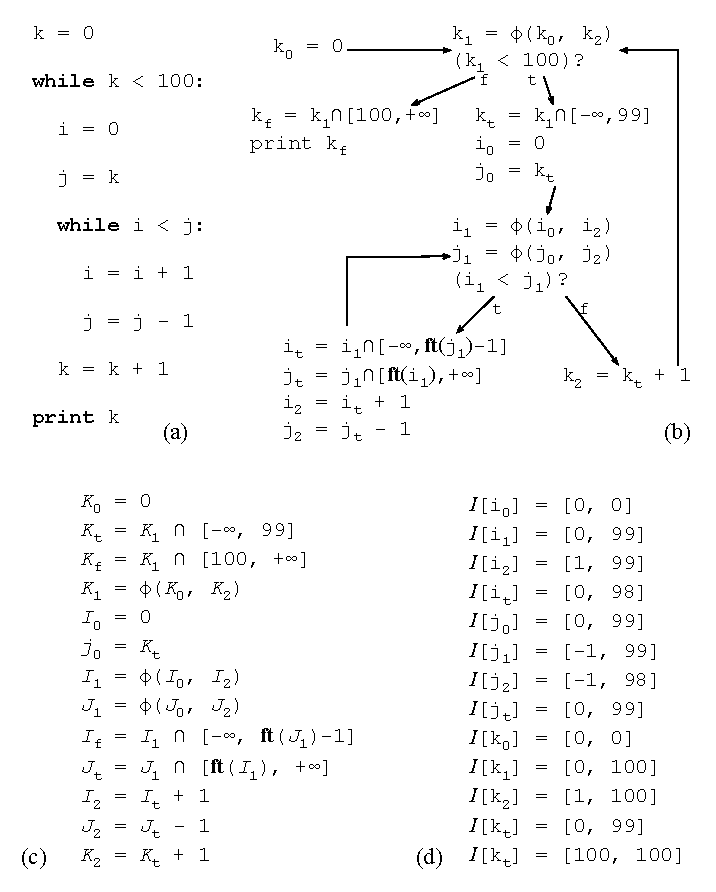
\includegraphics[width=\columnwidth]{images/ex_eSSA_cgo}
\end{center}
\caption{\label{fig:ex_eSSA_cgo}
(a) Example program.
(b) Control Flow Graph in SSA form.
(c) Constraints that we extract from the program.
(d) Possible solution to the range analysis problem.}
\end{figure}

\subsection{Widening, Future Resolution and Narrowing}
\label{sub:algo}

% The macro algorithm
The range analysis algorithm that we propose in this paper works in a number
of steps.
Firstly, we convert the program to an intermediate representation that gives
us subsidies to perform a sparse analysis.
We have tested our algorithm with two different representations, as we discuss
in Section~\ref{sub:splitting}.
Secondly, we extract constraints from the program representation.
Thirdly, we build a constraint graph, following the strategy pointed by
Su and Wagner~\cite{Su05}.
However, contrary to them, in a next phase we find the strongly connected
components in this graph, collapse them into super-nodes, and sort the
resulting digraph topologically.
Finally, for each strong component, we apply a three-phases approach to determine
the ranges of the variables.

\noindent
\textbf{Building the Constraint Graph. }
Given a set $\varset{C}$ of constraints, which define and/or use constraint
variables from a set $\varset{V}$, we build a constraint graph
$G = (\varset{C} \cup \varset{V}, E)$.
If variable $V \in \varset{V}$ is used in constraint $C \in \varset{C}$, then
we create an edge from $V$ to $C$.
If constraint $C \in \varset{C}$ defines variable $\varset{V} \in V$, then we
create an edge from $C$ to $V$.
Figure~\ref{fig:ex_graph} shows the constraint graph that we build for the
program in Figure~\ref{fig:ex_eSSA_cgo}(b).

\begin{figure}[t!]
\begin{center}
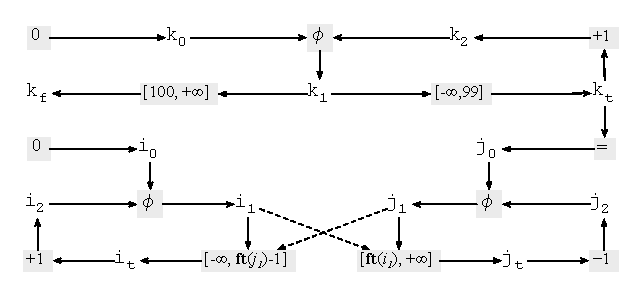
\includegraphics[width=\columnwidth]{images/ex_graph}
\end{center}
\caption{\label{fig:ex_graph}
The constraint graph that we build to the program in
Figure~\ref{fig:ex_eSSA_cgo}(b).}
\end{figure}


\subsection{Splitting Live Ranges after Uses of Variables}
\label{sub:splitting}

\section{The Dynamic Instrumentation Library}
\label{sec:dyn}


\section{Experimental Results}
\label{sec:exp}


\section{Related Work}
\label{sec:rel}


\section{Final Remarks}
\label{sec:rem}

\bibliographystyle{plain}
\bibliography{../references}

\end{document}
